\documentclass{article}

\usepackage{adjustbox} % adjust box for table
\usepackage{graphicx} % includes graphics
\usepackage{setspace} % spacing between lines
\usepackage{enumitem} % lists
\usepackage{amsmath} % math
\usepackage{lipsum} % lorem ipsum
\usepackage{paracol} % 2 columns page
\usepackage{sectsty} % need this to change section font-size
\usepackage[russian]{babel} % russian lang
\usepackage[fontsize=9pt]{fontsize} % sets default font-size
\usepackage[a4paper, total={7in, 9in}]{geometry} % margin for pages
\usepackage[colorlinks=true, allcolors=blue]{hyperref} % blue hyperlinks

\sectionfont{\fontsize{20}{20}\selectfont} % section font size
\setlength{\columnsep}{0.5cm} % separation between columns
\setlength{\parindent}{20pt} % spacing between paragraphs
\setlength{\thinmuskip}{5mu} % thinmuskip in formulas
\setlength{\medmuskip}{3mu} % medmuskip in formulas
%\setstretch{1.1} spacing between lines

\author{Ponomaryov Mikhail}
\date{December 2022}
%%%%%%%%%%%%%%%%%%%%%%%%%%%%%%%%%%%%%%%%%%%%%%%%%%%%%%%%%%%%%%%%%%%%%%%%%%%%%%%%%%%%%
\begin{document}
\setlength{\abovedisplayskip}{10pt} % skip above formulas
\setlength{\belowdisplayskip}{-2pt} % skip before formulas

\begin{paracol}{2}

\begin{flushleft}

\section*{Московский физико-технический институт}
\textbf{Ниже публикуются образцы вариантов всупительных письменных экзаменов по математике и физике в 1977 году.}

\subsection*{Математика}

\subsubsection*{Вариант 1}
\begin{enumerate}
    \item Решить уравнение 
    \[\sin(2x)-\sin^2(x)=2\sin(x)-4\cos(x)\].
    \item Решить неравенство
    \[\frac{5-4x}{3x^2-x-4}<4\].
    \item Решить уравнение 
    \[\lg^2(4-x)+\lg(4-x)\cdot\lg(x+\frac{1}{2})=2\lg^2(x+\frac{1}{2})\].
    \item Дорога проходит через пункты $A$ и $B$. Одновременно и в одном направлении
    выехали: из $A$ - мотоциклист (в направлении к $B$), из $B$ - велосипедист.
    Мотоциклист догнал велосипедиста на расстоянии a км от $B$. Если бы мотоциклист и велосипедист выехали одновременно из $A$ и $B$, то в момент прибытия мотоциклиста в B велосипедист отставал бы от него на $b$ км.
    Определить расстояние между пунктами $A$ и $B$ (скорости мотоциклиста и велосипедиста постоянны).
    \item Сторона основания $ABCD$ правильной пирамиды $SABCD$ имеет длину $a$, боковое ребро - длину $2a$. Рассматриваются отрезки с концами на диагонали $BD$ основания и боковом ребре $SC$, параллельные плоскости $SAD$.
    \begin{enumerate}
        \item Один из этих отрезков проведён через точку $M$ диагонали $BD$ такую, что $DM:DB=1:3$. Найти его длину.
        \item Найти наименьшую длину всех рассматриваемых отрезков.
    \end{enumerate}
    \item Графики функций $y = \frac{1}{x}$ и $y = 5 - \frac{3}{2} x$,                рассматривыемые в первой четверти координатной плоскости ($x > 0, y > 0$),       пересекаются в точках $A$ и $B$. Гипотенуза равнобедренного прямоугольного       треугольника параллельна оси $Ox$, две его вершины лежат на первом графике, а третья - на отрезке $AB$. Найти длины сторон треугольника.
\end{enumerate}

\end{flushleft}
%%%%%%%%%%%%%%%%%%%%%%%%%%%%%%%%%%%%%%%%%%%%%%%%%%%%%%%%%%%%%%%%%%%%%%%%%%%%%%%%%%%%%
\switchcolumn
\begin{flushleft}
\subsubsection*{Вариант 2}
\begin{enumerate}
    \item Решить уравнение
    \[\log_2\frac{x-7}{x-1}+log_2\frac{x-1}{x+1}=1\].
    \item Решить уравнение
    \[\frac{1}{\sin x}+\frac{1}{\sin(x-\frac{3\pi}{2})}=4\sin(x+\frac{5\pi}{4})\].
    \item В прямоугольном треугольнике $ABC$ катет BC имеет длину a и образует с     гипотенузой $AC$ угол $\alpha$. Точка $D$ расположена на катете $BC$ и имеет     наименьшую по сравнению с остальными точками отрезка $BC$ сумму квадратов          расстояний до прямых $AC$ и $AB$. Найти длину отрезка $BD$.
    \item Найти четыре числа, обладающих следующими свойствами:
    \begin{enumerate} 
        \item сумма первого и четвертого числа равна 14, а сумма второго и третьего равна 12;
        \item первое, второе и третье числа образуют в указанном порядке геометрическую прогрессию;
        \item второе, третье и четвертое числа образуют в указанном порядке арифметическую прогрессию.
    \end{enumerate} 
    \item Сторона основания правильной треугольной призмы $ABCA_1B_1C_1$ имеет длину $a$. Точка $D$ - середина ребра $AB$, точка $E$ лежит на ребре $A_1C_1$. Прямая $DE$ образует углы $\alpha$ и $\beta$ с плоскостями $ABC$ и $AA_1C_1C$ соответственно.\ Найти:
    \begin{enumerate}
        \item Высоту призмы;
        \item Радиус шара с центром на отрезке DE, касающегося плоскостей ABC и $AA_1C_1C$.
    \end{enumerate}
    \item Найти площадь фигуры, которая задаётся на координатной плоскости системой неравенств
    \begin{equation*}
        \begin{cases}
        \sqrt{3x^2+3y^2-3}\geq 2y+1,\\
        \ y+4\geq 2\sqrt{3}\ \lvert x \rvert
        \end{cases}
    \end{equation*}
\end{enumerate}

\subsection*{Физика}
\subsubsection*{Вариант 1}
\begin{enumerate}
    \item На покоящееся тело массы $m=5$ кг начинает действовать сила $\overrightarrow{F}$, величина которой убывает со временем по линейному закону до 0, как показано на рисунке 1. Какую скорость приобретает тело?
    \item Аквалангист затратил время $t=10$ мин на осмотр повреждения подводной части корабля. За это время давление в баллоне акваланга, первоначально равное 150 атм, упало на 20\%. После этого аквалангист \ldots
\end{enumerate}

\end{flushleft}

\end{paracol}
%%%%%%%%%%%%%%%%%%%%%%%%%%%%%%%%%%%%%%%%%%%%%%%%%%%%%%%%%%%%%%%%%%%%%%%%%%%%%%%%%%%%%
\newpage
\begin{paracol}{2}
\begin{flushleft}
    
\begin{figure}
  \centering
  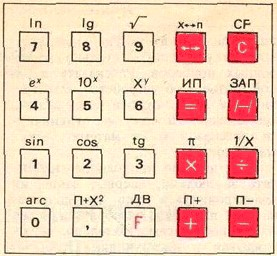
\includegraphics[scale=0.9]{pic.jpg}
  \caption{\label{fig:pic}Операции калькулятора}
\end{figure}
\lipsum[1-3]
\\
Picture \ref{fig:pic} - link example
\end{flushleft}
%%%%%%%%%%%%%%%%%%%%%%%%%%%%%%%%%%%%%%%%%%%%%%%%%%%%%%%%%%%%%%%%%%%%%%%%%%%%%%%%%%%%%
\switchcolumn
%%%%%%%%%%%%%%%%%%%%%%%%%%%%%%%%%%%%%%%%%%%%%%%%%%%%%%%%%%%%%%%%%%%%%%%%
\begin{table}[]
\begin{adjustbox}{width=\columnwidth,center}
\begin{tabular}{|l|llllllllll|l|}
\hline
\multicolumn{1}{|c|}{\begin{tabular}[c]{@{}c@{}}Кла-\\ виша\end{tabular}} &
  \multicolumn{10}{c|}{Табло} &
  \multicolumn{1}{c|}{Пояснения} \\ \hline
 &
  \multicolumn{1}{l|}{} &
  \multicolumn{1}{l|}{} &
  \multicolumn{1}{l|}{} &
  \multicolumn{1}{l|}{} &
  \multicolumn{1}{l|}{} &
  \multicolumn{1}{l|}{} &
  \multicolumn{1}{l|}{} &
  \multicolumn{1}{l|}{} &
  \multicolumn{1}{l|}{} &
  0, &
  \multicolumn{1}{c|}{\begin{tabular}[c]{@{}c@{}}начальное состояние\\ (переключатель "вкл".)\end{tabular}} \\ \hline
4 &
  \multicolumn{1}{l|}{} &
  \multicolumn{1}{l|}{} &
  \multicolumn{1}{l|}{} &
  \multicolumn{1}{l|}{} &
  \multicolumn{1}{l|}{} &
  \multicolumn{1}{l|}{} &
  \multicolumn{1}{l|}{} &
  \multicolumn{1}{l|}{} &
  \multicolumn{1}{l|}{} &
  8, &
   \\ \hline
8 &
  \multicolumn{1}{l|}{} &
  \multicolumn{1}{l|}{} &
  \multicolumn{1}{l|}{} &
  \multicolumn{1}{l|}{} &
  \multicolumn{1}{l|}{} &
  \multicolumn{1}{l|}{} &
  \multicolumn{1}{l|}{} &
  \multicolumn{1}{l|}{} &
  \multicolumn{1}{l|}{4} &
  8, &
   \\ \hline
, &
  \multicolumn{1}{l|}{} &
  \multicolumn{1}{l|}{} &
  \multicolumn{1}{l|}{} &
  \multicolumn{1}{l|}{} &
  \multicolumn{1}{l|}{} &
  \multicolumn{1}{l|}{} &
  \multicolumn{1}{l|}{} &
  \multicolumn{1}{l|}{} &
  \multicolumn{1}{l|}{4} &
  8, &
  \multicolumn{1}{c|}{\begin{tabular}[c]{@{}c@{}}отделение\\ (фиксация)\\ целой части\\ вводимого\\ числа\end{tabular}} \\ \hline
5 &
  \multicolumn{1}{l|}{} &
  \multicolumn{1}{l|}{} &
  \multicolumn{1}{l|}{} &
  \multicolumn{1}{l|}{} &
  \multicolumn{1}{l|}{} &
  \multicolumn{1}{l|}{} &
  \multicolumn{1}{l|}{} &
  \multicolumn{1}{l|}{4} &
  \multicolumn{1}{l|}{8,} &
  5 &
   \\ \hline
8 &
  \multicolumn{1}{l|}{} &
  \multicolumn{1}{l|}{} &
  \multicolumn{1}{l|}{} &
  \multicolumn{1}{l|}{} &
  \multicolumn{1}{l|}{} &
  \multicolumn{1}{l|}{4} &
  \multicolumn{1}{l|}{8,} &
  \multicolumn{1}{l|}{5} &
  \multicolumn{1}{l|}{8} &
  7 &
   \\ \hline
(-) &
  \multicolumn{1}{l|}{-} &
  \multicolumn{1}{l|}{} &
  \multicolumn{1}{l|}{} &
  \multicolumn{1}{l|}{} &
  \multicolumn{1}{l|}{} &
  \multicolumn{1}{l|}{4} &
  \multicolumn{1}{l|}{8,} &
  \multicolumn{1}{l|}{5} &
  \multicolumn{1}{l|}{8} &
  7 &
  \multicolumn{1}{c|}{\begin{tabular}[c]{@{}c@{}}изменение знака числа\\ (умножение на -1)\end{tabular}} \\ \hline
\end{tabular}
\end{adjustbox}
\end{table}
%%%%%%%%%%%%%%%%%%%%%%%%%%%%%%%%%%%%%%%%%%%%%%%%%%%%%%%%%%%%%%%%%%%%%%
\end{paracol}

\end{document}